\begin{question}[section=2,name={24.7.2013},mode=exm,type=bsp,tags={20130724}]
Eine fremderregte Gleichstrommaschine hat folgende Daten.\\
\begin{tabular}{L{2cm}l}
$I_{N}$ \dotfill &$200~A$\\
$k_1 \phi_N$ \dotfill & $15~Vs$ \\
$n_N$ \dotfill & $1960~\frac{U}{min}$\\
$n_0$ \dotfill & $2000~\frac{U}{min}$
\end{tabular}
\begin{compactenum}
\item Berechnen Sie den Ankerwiderstand der Gleichstrommaschine. (\addpoints{2})
\item Wie groß ist das Nennmoment der Gleichstrommaschine. (\addpoints{1})
\item Die Gleichstrommaschine wird mit konstanter Ankerspannung $U_A = 300~V$ versorgt, es liegt Nennerregung an. Berechnen Sie die Drehzahl in Abhängigkeit des Moments $n=f(M_i)$. (\addpoints{3})
\item Skizzieren Sie für den gegebenen Motor diesen Verlauf im Bereich $\pm M_N$. (\addpoints{1})
\item Das Feld wird nun auf die Hälfte der Nennerregung eingestellt. Wie groß ist nun das mit Nennstrom maximal erreichbare Drehmoment. (\addpoints{1})
\item Die Gleichstrommaschine wird mit konstanter Ankerspannung $U_A = 300~V$ versorgt, jedoch mit halber Nennerregung. Berechnen Sie die Drehzahl in Abhängigkeit des Moments $n=f(M_i)$. (\addpoints{2})
\item Skizzieren Sie diesen Verlauf im Bereich $\pm M_N$. (\addpoints{1})
\item Berechnen Sie den Wirkungsgrad der Gleichstrommaschine. (\addpoints{1})
\end{compactenum}
\end{question}
\begin{solution}
\begin{compactenum}
\item Um den Ankerwiderstand berechnen zu können wird die Ankernennspannung benötigt. Diese errechnet sich aus der Spannungskonstante mit der Leerlaufdrehzahl. Anschließend wird mit (\ref{glg:Ankerspannungsgleichung}) der Ankerwiderstand durch umformen errechnet.\\
\begin{align}
U_{A,N} &= \frac{k \Phi}{2 \pi} \cdot \frac{2000}{60} 2 \pi = 500~V\\
R_A &= \frac{U_{A,N} - \frac{k \Phi}{2 \pi} \cdot \frac{n_N}{60} 2 \pi}{I_A}=50~m \Omega\\
k^{'}\Phi&= \frac{k \Phi}{2 \pi}
\end{align}
\item Das Moment errechnet sich mit (\ref{glg:Ankermoment}).\\
\begin{equation}
M_N=\frac{k \Phi}{2 \pi} \cdot I_N =477,46~Nm
\end{equation}
\item Das Ankermoment (\ref{glg:Ankermoment}) wird auf $I_A$ umgeformt und in (\ref{glg:Ankerspannungsgleichung}) eingesetzt und auf $\Omega$ umgeformt und Anschließend mit $\frac{60}{2 \pi}$ mulitpliziert um auf $n$ in Umdrehungen pro Minute zu kommen.
\begin{equation}
n(M_i) = \frac{U_A - R_A \frac{M_i}{k^{'} \Phi}}{k^{'}\Phi} \cdot \frac{60}{2 \pi}=1200-0,0837 \cdot M_i
\end{equation}
\item \textbf{TODO:} Programmiere oder zeichne die Grafik und scan sie ein und lade sie hoch!
%\begin{figure}[H]
%\center
%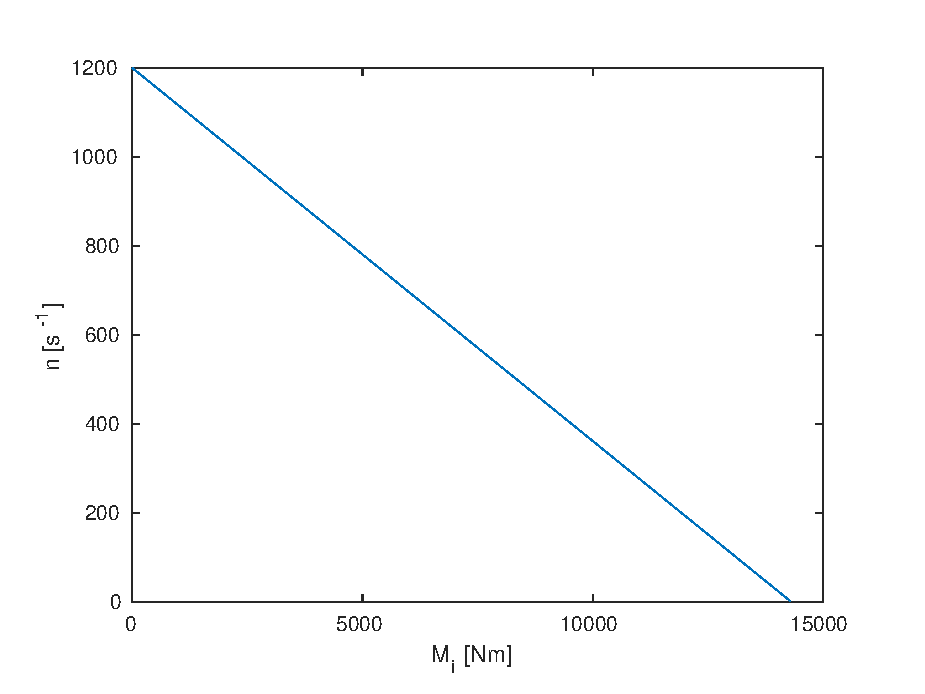
\includegraphics[width=0.5\textwidth]{201307242_4}
%\caption{Drehzahl in Abhängigkeit vom Drehmoment}
%\end{figure}
\item Das Moment errechnet sich mit (\ref{glg:Ankermoment}), wobei die Hälfte der Erregung $k^{'} \Phi$ eingesetzt wird.
\begin{equation}
M_{\frac{N}{2}} = \frac{k^{'}\Phi}{2} I_A =238,73~Nm
\end{equation}
\item Das Ankermoment (\ref{glg:Ankermoment}) wird auf $I_A$ umgeformt und in (\ref{glg:Ankerspannungsgleichung}) eingesetzt und auf $\Omega$ umgeformt, wobei die Hälfte der Erregung $k^{'} \Phi$ eingesetzt wird und Anschließend mit $\frac{60}{2 \pi}$ mulitpliziert wird um auf $n$ in Umdrehungen pro Minute zu kommen.
\begin{equation}
n(M_i) = \frac{U_A - R_A \frac{2 M_i}{k^{'} \Phi}}{k^{'}\Phi} \cdot 2 \cdot \frac{60}{2 \pi} =2400-0,335 \cdot M_i
\end{equation}
\item \textbf{TODO:} Programmiere oder zeichne die Grafik und scan sie ein und lade sie hoch!
%\begin{figure}[H]
%\center
%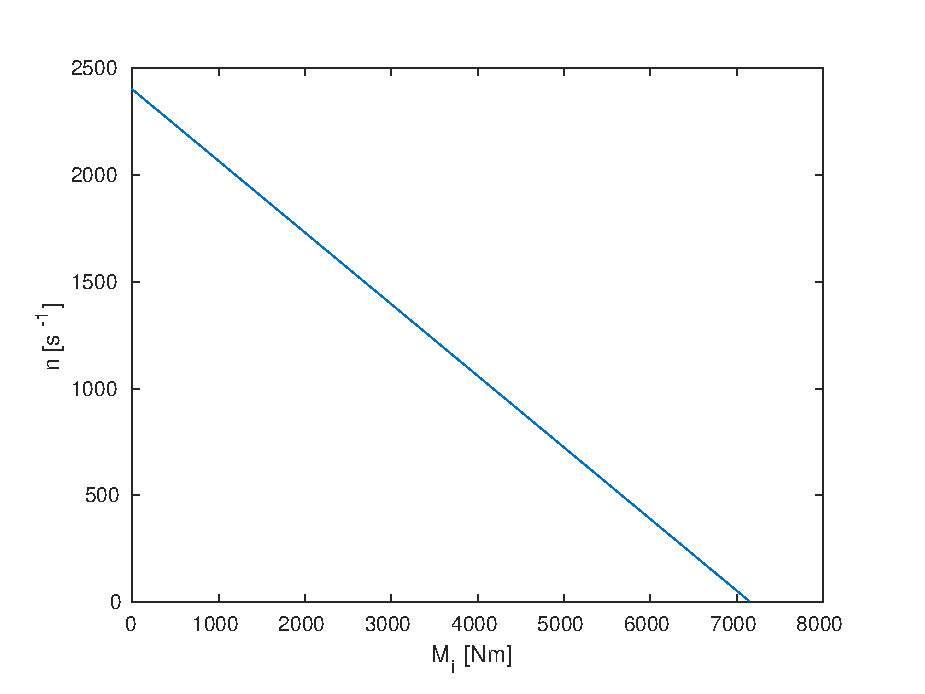
\includegraphics[width=0.5\textwidth]{201307242_6}
%\caption{Drehzahl in Abhängigkeit vom Drehmoment}
%\end{figure}
\item In (\ref{glg:Wirkungsgrad}) einsetzen. Es ergeben sich drei Wirkungsgrade. (Nennwirkungsgrad, Wirkungsgrad bei $300~V$ und Nennmoment, Wirkungsgrad bei $300~V$ 
Aus der allgemeinen Wirkungsgradgleichung:
\[\eta = \frac{P_{out}}{P_{in}}\]
\begin{align}
\eta_N &= \frac{M_N \Omega_N}{U_{A,N} I_A} = 0,98\\
\eta_1 &= \frac{M_N \Omega_{M_N}}{300 \cdot I_A} = 0,967\\
\eta_2 &= \frac{M_{N/2} \Omega_{M_N}}{300 \cdot I_A} = 0,963
\end{align}
\end{compactenum}
\end{solution}